\documentclass[border=10pt]{standalone}
\usepackage{pgfplots}
\pgfplotsset{compat=1.18}

\begin{document}
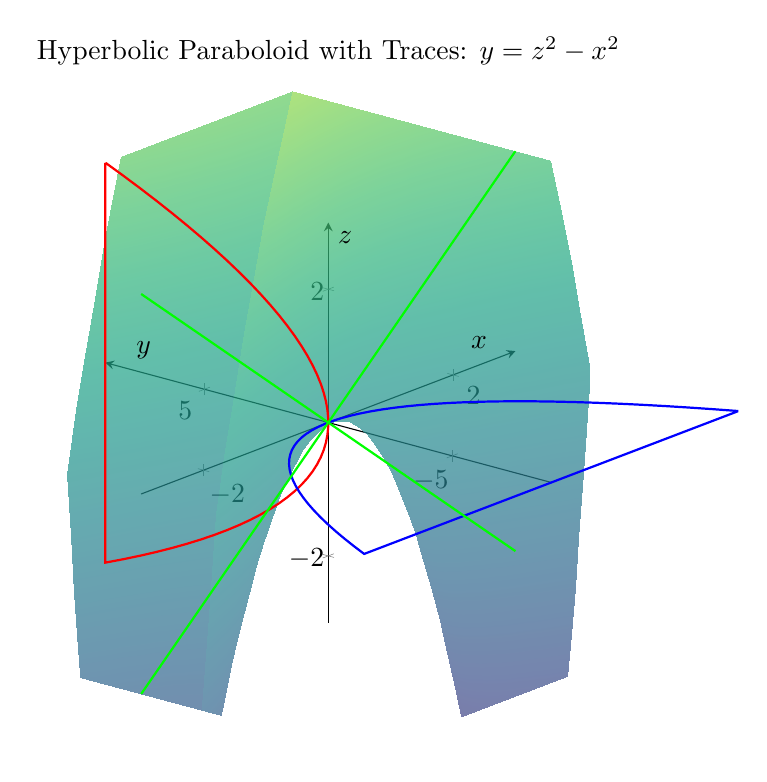
\begin{tikzpicture}
\begin{axis}[
    xlabel=$x$,
    ylabel=$y$,
    zlabel=$z$,
    title={Hyperbolic Paraboloid with Traces: $y = z^2 - x^2$},
    view={-50}{25},
    colormap/viridis,
    grid=none,
    axis lines=center,
    domain=-3:3,
    y domain=-3:3,
    samples=40,
    samples y=40,
    zmin=-3, zmax=3,
    xmin=-3, xmax=3,
    ymin=-9, ymax=9,
    width=12cm,
    height=10cm,
]
% Main surface
\addplot3[surf, opacity=0.7, shader=interp] {y^2 - x^2};

% Trace x=0 (red parabola)
\addplot3[red, thick, domain=-3:3, samples=50] ({0}, {x^2}, {x});

% Trace z=0 (blue parabola)
\addplot3[blue, thick, domain=-3:3, samples=50] ({x}, {-x^2}, {0});

% Trace y=0 (green lines)
\addplot3[green, thick, domain=-3:3, samples=50] ({x}, {0}, {x});
\addplot3[green, thick, dashed, domain=-3:3, samples=50] ({x}, {0}, {-x});

\end{axis}
\end{tikzpicture}
\end{document}